\chapter{Simulaci\'{o}n Computacional}
\section{Modelo de vSGLT con C-$\alpha$}
\begin{figure}
 \centering
  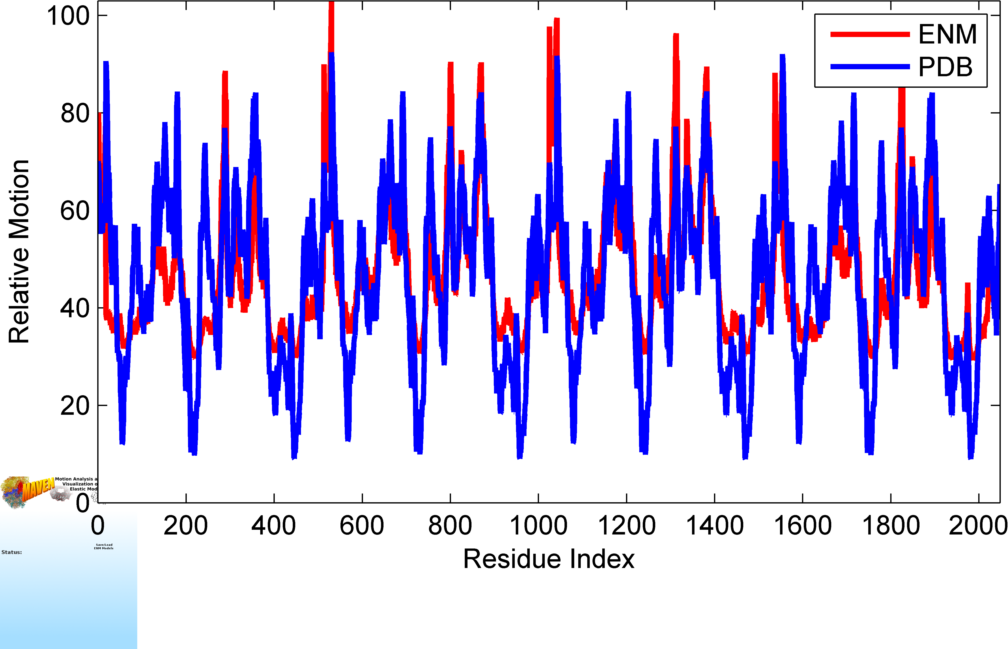
\includegraphics[scale=0.3]{./Kap4/ANM/Ca/BF_plot_100.png}
 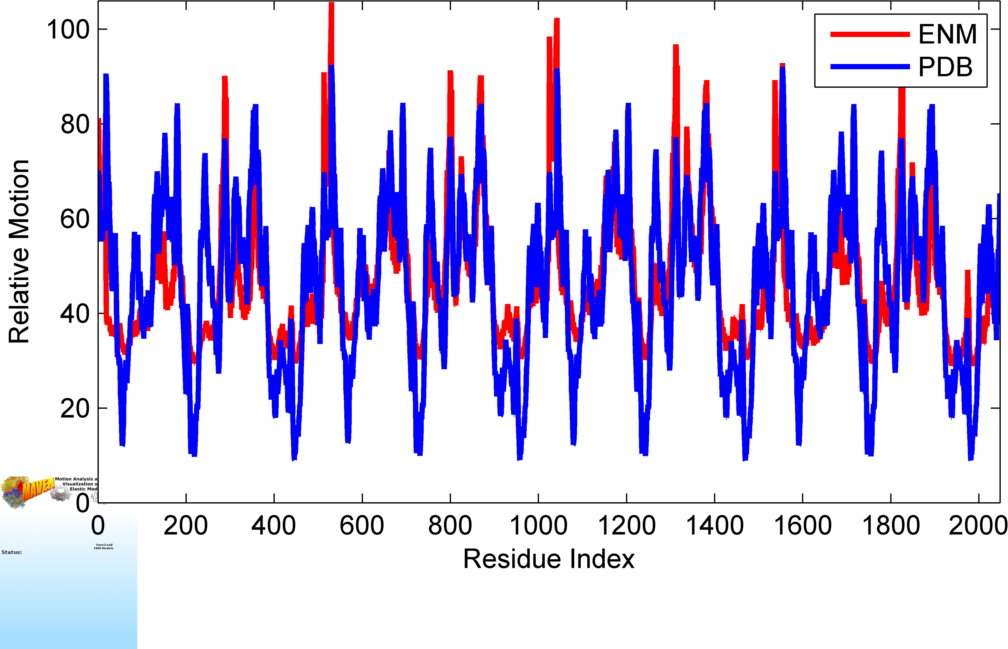
\includegraphics[scale=0.3]{./Kap4/ANM/Ca/BF_plot.png}
 \caption{ANM para $R_c=8\AA$ usando a) los primeros 100 modos. b) usando todos los modos}
\end{figure}
\begin{figure}
 \centering
  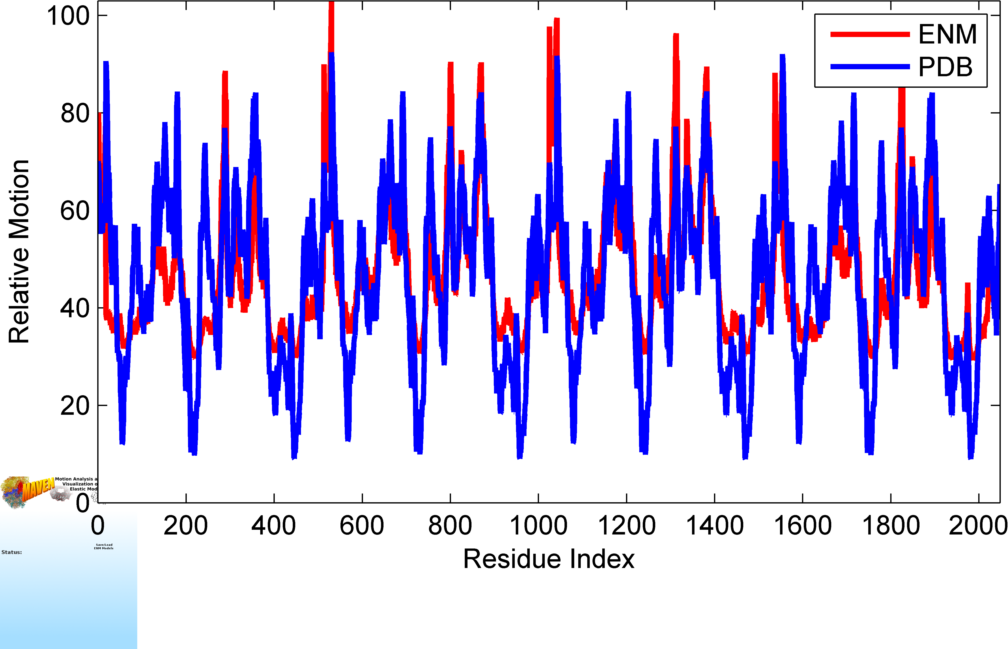
\includegraphics[scale=0.3]{./Kap4/ANM/Ca/BF_plot_100.png}
 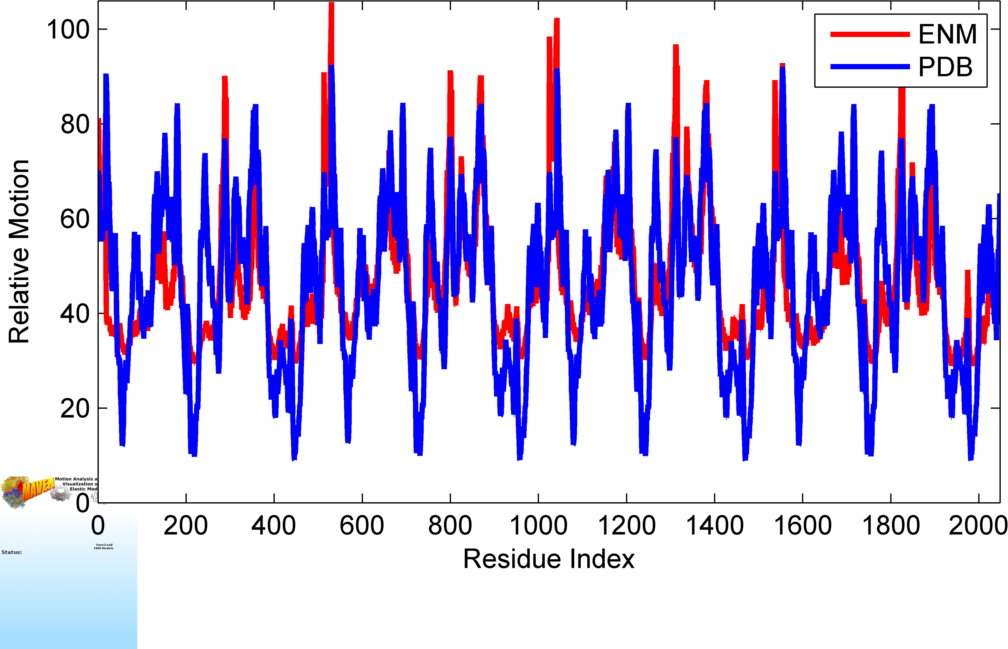
\includegraphics[scale=0.3]{./Kap4/ANM/Ca/BF_plot.png}
 \caption{ANM para $R_c=8\AA$ usando a) los primeros 100 modos. b) usando todos los modos}
\end{figure}
\section{Modelo de vSGLT con C-$\alpha$ y Galactosa}

\section{Mutante K294a de vSGLT con C-$\alpha$}